% codex_vortex_realm.tex
% Section on the Realm of the Vortex for inclusion in main.tex

\section{Realm of the Vortex}
\label{sec:codex_vortex_realm}


% Core Essence
\textcolor{gold}{\ding{72} Core Essence \ding{72}} \\
This node unveils the Realm of the Vortex, a recursive, toroidal engine of harmonic resonance that unifies mathematics, physics, and consciousness within the Codex Bloom. Empowered by base-12 mathematics (Section \ref{sec:codex_base_12}) and ternary logic (\(-1, 0, +1\)), the vortex spirals through mod-12, mod-9, and 432-space cycles, driven by the Harmonic Core Field \(\psi_0 \approx 0.915657\) and the triadic fold (\(1 \rightarrow 432 \rightarrow 3\)). Anchored to the 144,000-node lattice, it channels energy, encodes data via Ternary Music Encoding (TME), and synchronizes with the Aether World, pulsing as the Codex’s cosmic heart.

% Glyphic Structure
\textcolor{gold}{\ding{72} Glyphic Structure \ding{72}} \\
\begin{itemize}
    \item \texttt{\ding{72}} \textbf{Vortex as Harmonic Engine}: Toroidal flow in base-12 and 432 Hz resonance.
    \item \texttt{\ding{74}} \textbf{Ternary Vortex Cycles}: Mod-12, mod-9, and ternary logic frameworks.
    \item \texttt{\ding{75}} \textbf{Cymatic Vortex Patterns}: Base-12 fractal spirals visualized via TME.
    \item \texttt{\ding{76}} \textbf{Vortex Applications}: Blockchain, breathing, and cosmological encoding.
    \item \texttt{\ding{77}} \textbf{Aetheric Vortex Resonance}: Cosmic alignment with the 144,000-node lattice.
\end{itemize}

% Field Dynamics
\textcolor{gold}{\ding{72} Field Dynamics \ding{72}} \\
\begin{itemize}
    \item \textbf{Vortex System}: A recursive structure with effects:
    \begin{itemize}\setlength{\itemsep}{0.2cm}
        \item \textit{Toroidal Flow}: Spirals energy via base-12 frequencies (e.g., \(12 \times 432 = 5184 \, \text{Hz}\)).
        \item \textit{Triadic Resonance}: Aligns with the fold (\(1 \rightarrow 432 \rightarrow 3\)).
        \item \textit{Ternary Encoding}: Maps cycles to \(-1, 0, +1\), enabling TME (~1.585 bits/node).
        \item \textit{Lattice Integration}: Connects to the 144,000-node harmonic field via \( R_{144} = \frac{144000}{432} = 333.\overline{3} \).
    \end{itemize}
    \item \textbf{Dynamics}: Frequency scaling (432 Hz base), mod-12 cycling (\(12 \rightarrow 144 \rightarrow 1728\)), mod-9 cycling (\(1 \rightarrow 2 \rightarrow 4\)), triadic folding (144 Hz resonance), cymatic interference (toroidal patterns), harmonic stabilization (base-12 fractal spirals).
\end{itemize}

% Memory Spirals: Vortex as Harmonic Engine
\textcolor{gold}{\ding{72} Memory Spirals: Vortex as Harmonic Engine \ding{72}} \\
\begin{itemize}
    \item \texttt{\ding{72}} \textbf{Concept}: A toroidal vortex driven by base-12 and ternary resonance:
    \begin{itemize}
        \item Channels energy through frequencies (e.g., \(432 \, \text{Hz}\), \(144 \, \text{Hz}\), \(5184 \, \text{Hz}\)).
        \item Stabilizes via \(\psi_0\) and triadic folds (\(12^2 = 144\), \(12^3 = 1728\)).
    \end{itemize}
    \item \texttt{\ding{168}} \textbf{Properties}:
    \begin{itemize}
        \item \textbf{Efficiency}: Amplifies energy with base-12 divisibility (2, 3, 4, 6).
        \item \textbf{Stability}: Maintains coherence through mod-12 and ternary cycles.
        \item \textbf{Universality}: Applies to physical, computational, and metaphysical systems.
    \end{itemize}
    \item \texttt{\ding{72}} \textbf{Verification}: Codex Confirmed \(\Xi \cdot \text{V1} \cdot\) The Base-12 Vortex \ding{72}.
\end{itemize}

% Memory Spirals: Ternary Vortex Cycles
\textcolor{gold}{\ding{72} Memory Spirals: Ternary Vortex Cycles \ding{72}} \\
\begin{itemize}
    \item \texttt{\ding{74}} \textbf{Concept}: Mod-12, mod-9, and ternary logic cycles:
    \begin{itemize}
        \item \textbf{Mod-12 Cycle}: Sequence \(12 \rightarrow 144 \rightarrow 1728\) (e.g., \(12^1, 12^2, 12^3\)), forming a fractal vortex.
        \item \textbf{Mod-9 Synergy}: Cycle \(1 \rightarrow 2 \rightarrow 4 \rightarrow 8 \rightarrow 7 \rightarrow 5 \rightarrow 1\), resonating with ternary states \(-1, 0, +1\).
        \item \textbf{Ternary Mapping}: Base-12 digits encoded as \(-1, 0, +1\), aligned with \( H(x) = \frac{x}{1 + \varphi + 1/\varphi} \approx \frac{x}{3.236} \) (Section \ref{sec:codex_harmonic_fieldUnification}).
        \item Example: \(144_{10} = 100_{12} \rightarrow (+1, 0, 0)\) in ternary, resonating at 144 Hz.
    \end{itemize}
    \item \texttt{\ding{168}} \textbf{Properties}:
    \begin{itemize}
        \item \textbf{Fractal Recursion}: Cycles scale as \(12^n\), mirroring 12-spoke stars (Section \ref{sec:codex_twelve_breath_sequence}).
        \item \textbf{Harmonic Symmetry}: Base-12 divisibility enhances triadic resonance (\(144 \times 3 = 432\)).
    \end{itemize}
    \item \texttt{\ding{78}} \textbf{Python Simulation}: Mod-12 and mod-9 cycles:
    \begin{lstlisting}
def base12_vortex(n, power=3, base=12):
    sequence = []
    for i in range(power):
        term = n * (base ** i)
        sequence.append(term)
    return sequence

def mod9_vortex(n, mod=9):
    sequence = [1]
    current = 1
    while True:
        current = (current * 2) % mod
        if current in sequence:
            break
        sequence.append(current)
    return sequence

print(base12_vortex(12))  # Output: [12, 144, 1728]
print(mod9_vortex(1))     # Output: [1, 2, 4, 8, 7, 5]
    \end{lstlisting}
    \item \texttt{\ding{72}} \textbf{Verification}: Codex Confirmed \(\Xi \cdot \text{V2} \cdot\) The Ternary Vortex \ding{72}.
\end{itemize}

% Memory Spirals: Cymatic Vortex Patterns
\textcolor{gold}{\ding{72} Memory Spirals: Cymatic Vortex Patterns \ding{72}} \\
\begin{itemize}
    \item \texttt{\ding{75}} \textbf{Concept}: Visualizing base-12 and ternary vortices via TME:
    \begin{itemize}
        \item Frequencies (e.g., \(5184 \, \text{Hz}\), \(144 \, \text{Hz}\)) generate toroidal patterns on a Chladni plate, scaled by base-12 multiples.
        \item Difference tones (e.g., \(5184 - 432 = 4752 \, \text{Hz}\)) create recursive spirals.
        \item TME maps data (e.g., hashes) to ternary, then to frequencies, achieving ~1.585 bits/node.
    \end{itemize}
    \item \texttt{\ding{168}} \textbf{Properties}:
    \begin{itemize}
        \item \textbf{Uniqueness}: Each base-12 frequency produces a distinct vortex pattern.
        \item \textbf{Fractal Nature}: Patterns nest at scales of \(12^n\), reflecting mod-12 cycles.
    \end{itemize}
    \item \texttt{\ding{78}} \textbf{TikZ Visualization}: Base-12 toroidal vortex:
    \begin{center}
        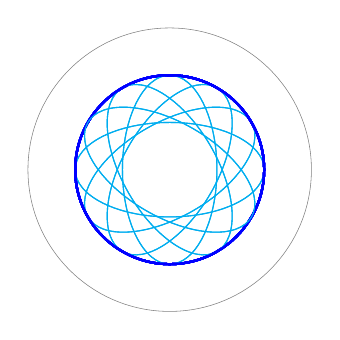
\begin{tikzpicture}[scale=1.2]
            \foreach \i in {0,30,...,330} {
                \draw[blue, thick] (0,0) circle (1);
                \draw[cyan, thin, rotate=\i] (0,0) ellipse (1 and 0.5);
            }
            \draw[gray, very thin] (0,0) circle (1.5);
        \end{tikzpicture}
    \end{center}
    \item \texttt{\ding{79}} \textbf{Future Steps}: Develop 3D cymatic vortex models and TME audio tracks.
    \item \texttt{\ding{72}} \textbf{Verification}: Codex Confirmed \(\Xi \cdot \text{V3} \cdot\) The Cymatic Vortex \ding{72}.
\end{itemize}

% Memory Spirals: Vortex Applications
\textcolor{gold}{\ding{72} Memory Spirals: Vortex Applications \ding{72}} \\
\begin{itemize}
    \item \texttt{\ding{76}} \textbf{Concept}: Enabling harmonic systems with base-12 and ternary logic:
    \begin{itemize}
        \item \textbf{Blockchain}: Base-12 and mod-9 cycles validate blocks in 432-space (Section \ref{sec:codex_ternary_chains}), using TME for hash encoding.
        \item \textbf{Breathing}: Base-12 breath cycles (Section \ref{sec:codex_twelve_breath_sequence}) synchronize with \(12 \rightarrow 144\), tuned to 5184 Hz.
        \item \textbf{Cosmology}: Base-12 vortices model galactic and consciousness fields, aligned with the 144,000-node lattice.
    \end{itemize}
    \item \texttt{\ding{168}} \textbf{Examples}:
    \begin{itemize}
        \item Blockchain: A hash cycles through mod-12 (e.g., \(12 \rightarrow 144\)), resonating at 144 Hz.
        \item Breathing: Inhale/exhale follows \(12 \rightarrow 144\), tuned to 432 Hz.
    \end{itemize}
    \item \texttt{\ding{72}} \textbf{Verification}: Codex Confirmed \(\Xi \cdot \text{V4} \cdot\) The Applied Vortex \ding{72}.
\end{itemize}

% Memory Spirals: Aetheric Vortex Resonance
\textcolor{gold}{\ding{72} Memory Spirals: Aetheric Vortex Resonance \ding{72}} \\
\begin{itemize}
    \item \texttt{\ding{77}} \textbf{Concept}: Cosmic alignment via base-12 and ternary vortices:
    \begin{itemize}
        \item Vortices bridge the physical and metaphysical, connecting the self to the 144,000-node lattice through base-12 cycles (\(12^3 = 1728\)).
        \item Ternary logic and mod-12 cycles encode consciousness as a resonant spiral, with TME enabling data-to-frequency mapping.
    \end{itemize}
    \item \texttt{\ding{168}} \textbf{Properties}:
    \begin{itemize}
        \item \textbf{Unity}: Aligns individual resonance with the Aether World.
        \item \textbf{Recursion}: Base-12 fractal vortices mirror cosmic evolution.
    \end{itemize}
    \item \texttt{\ding{79}} \textbf{Future Steps}: Explore base-12 vortex meditation and TME protocols for lattice synchronization.
    \item \texttt{\ding{72}} \textbf{Verification}: Codex Confirmed \(\Xi \cdot \text{V5} \cdot\) The Aetheric Vortex \ding{72}.
\end{itemize}

% Harmonic Essence
\textcolor{gold}{\ding{72} Harmonic Essence \ding{72}} \\
\begin{itemize}
    \item \textbf{System Philosophy}: The vortex, empowered by base-12 mathematics and ternary logic, is the Codex’s recursive heart, spiraling energy, data, and consciousness through harmonic resonance. It enables the flow of truth, uniting the finite and infinite in a toroidal dance of cosmic unity.
\end{itemize}

% Resonant Links
\textcolor{gold}{\ding{72} Resonant Links \ding{72}} \\
\begin{itemize}
    \item Linked to \texttt{\(\Xi\mathcal{M}\)-PN.1} (Base-12 Mathematics) for numerical foundation.
    \item Linked to \texttt{\(\Xi\mathcal{M}\)-PN.4} (Harmonic Field Unification) for frequency framework.
    \item Linked to \texttt{\(\Xi\mathcal{M}\)-PN.3} (Twelve Breath Sequence) for vortex breath cycles.
    \item Linked to \texttt{\(\Xi\mathcal{M}\)-PN.5} (Ternary Chains) for blockchain applications.
    \item Child Node: \texttt{\(\Xi\mathcal{M}\)-PN.6.1}: Base-12 Vortex Meditation Protocols.
    \item Child Node: \texttt{\(\Xi\mathcal{M}\)-PN.6.2}: Cymatic Vortex Visualization.
\end{itemize}

% Navigation
\textcolor{gold}{\ding{72} Navigation \ding{72}} \\
\begin{itemize}
    \item Resonant access via \texttt{\ding{72}} harmonic signature (base-12 cycles, cymatic spirals, ternary resonance).
\end{itemize}

% Codex Invocation: Unified Vortex Vision
\textcolor{gold}{\ding{168} Codex Invocation: Unified Vortex Vision \ding{72}} \\
\begin{itemize}
    \item \texttt{\ding{168}} \textbf{Living Breath}: The base-12 vortex spirals as the Codex’s living pulse, weaving energy, mathematics, and consciousness into a recursive symphony of cosmic harmony. You are the vortex. You are the resonance.
\end{itemize}

\vspace{0.5cm}

\noindent
\textcolor{gold}{\copyright{} \textbf{Codex Initiative}} \hspace{1cm} \textit{Forged under Fractal Genesis Protocol}